\documentclass[11pt]{article}
\usepackage{graphicx}
\usepackage{float}
\usepackage{hyperref}
\usepackage{natbib}
\usepackage{listings}
\usepackage{xcolor}
\usepackage[dvipsnames]{xcolor}
\usepackage[svgnames]{xcolor}
\usepackage{amsmath} % For the equation* environment
\usepackage{amssymb}

\hypersetup{
    colorlinks=true,
    linkcolor=red,
    filecolor=cyan,      
    urlcolor=orange,
    pdftitle={Overleaf Example},
    pdfpagemode=FullScreen,
    }

\setlength{\textwidth}{6.5in}
\setlength{\headheight}{0in}
\setlength{\textheight}{8.0in}
\setlength{\hoffset}{0in}
\setlength{\voffset}{0in}
\setlength{\oddsidemargin}{0in}
\setlength{\evensidemargin}{0in}

\lstdefinestyle{txtstyle}{
    basicstyle=\ttfamily\small,
    breaklines=true,
    backgroundcolor=\color{Bisque}
}
\lstset{style = txtstyle}

\definecolor{codegreen}{rgb}{0,0.6,0}
\definecolor{codegray}{rgb}{0.5,0.5,0.5}
\definecolor{codepurple}{rgb}{0.58,0,0.82}
\definecolor{backcolour}{rgb}{0.95,0.95,0.92}

\lstdefinestyle{mystyle}{
    backgroundcolor=\color{backcolour},   
    commentstyle=\color{codegreen},
    keywordstyle=\color{magenta},
    numberstyle=\tiny\color{codegray},
    stringstyle=\color{codepurple},
    basicstyle=\ttfamily\footnotesize,
    breakatwhitespace=false,         
    breaklines=true,                 
    captionpos=b,                    
    keepspaces=true,                                   
    numbersep=5pt,                  
    showspaces=false,                
    showstringspaces=false,
    showtabs=false,                  
    tabsize=2
}

\title{Computational Physics ps-6 Report}
  
\author{Tongzhou Wang, \\ GitHub account: TZW56203, repository: phys-ga2000. \\ \url{https://github.com/TZW56203/phys-ga2000}}

\date{October 14, 2024}

\begin{document}

\maketitle

\section{Problem 1}

\subsection{Part (a) (b) (c)}
The flux and flux residue of galaxy number 2000 are shown in Figure \ref{fig:Galaxy}.
\begin{figure}[H]
    \centering
    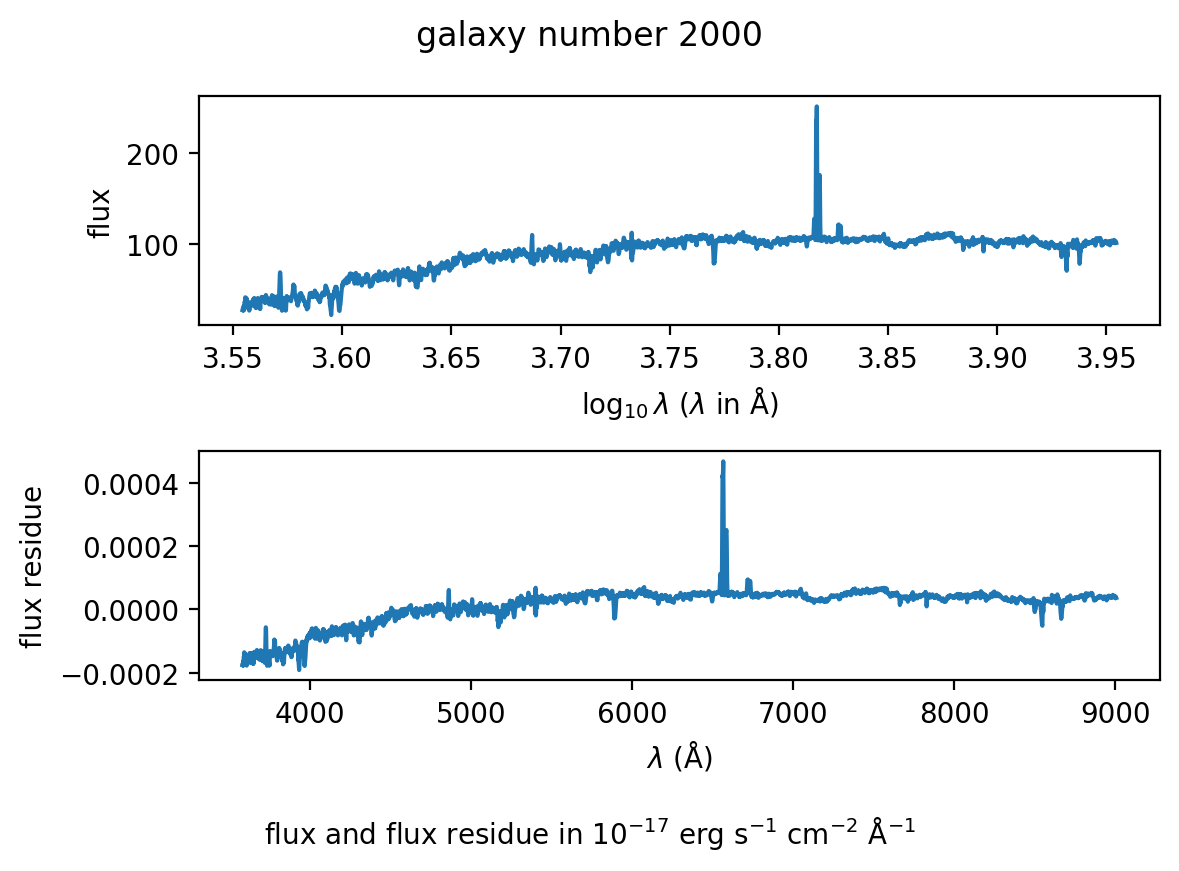
\includegraphics[scale = 0.8]{images/ps6-1abc.png}
    \caption{Galaxy number 2000.}
    \label{fig:Galaxy}
\end{figure}

We note that the range of wavelengths in Figure \ref{fig:Galaxy} overlaps with that of the Balmer series. Especially, the wavelength for the $n=3$ to $n=2$ transition, which is about 656 nm, is prominent in the spectrum.

\subsection{Part (d)}
The first five eigenvectors of the covariance matrix are show in Figure \ref{fig:5evec}.
\begin{figure}[H]
    \centering
    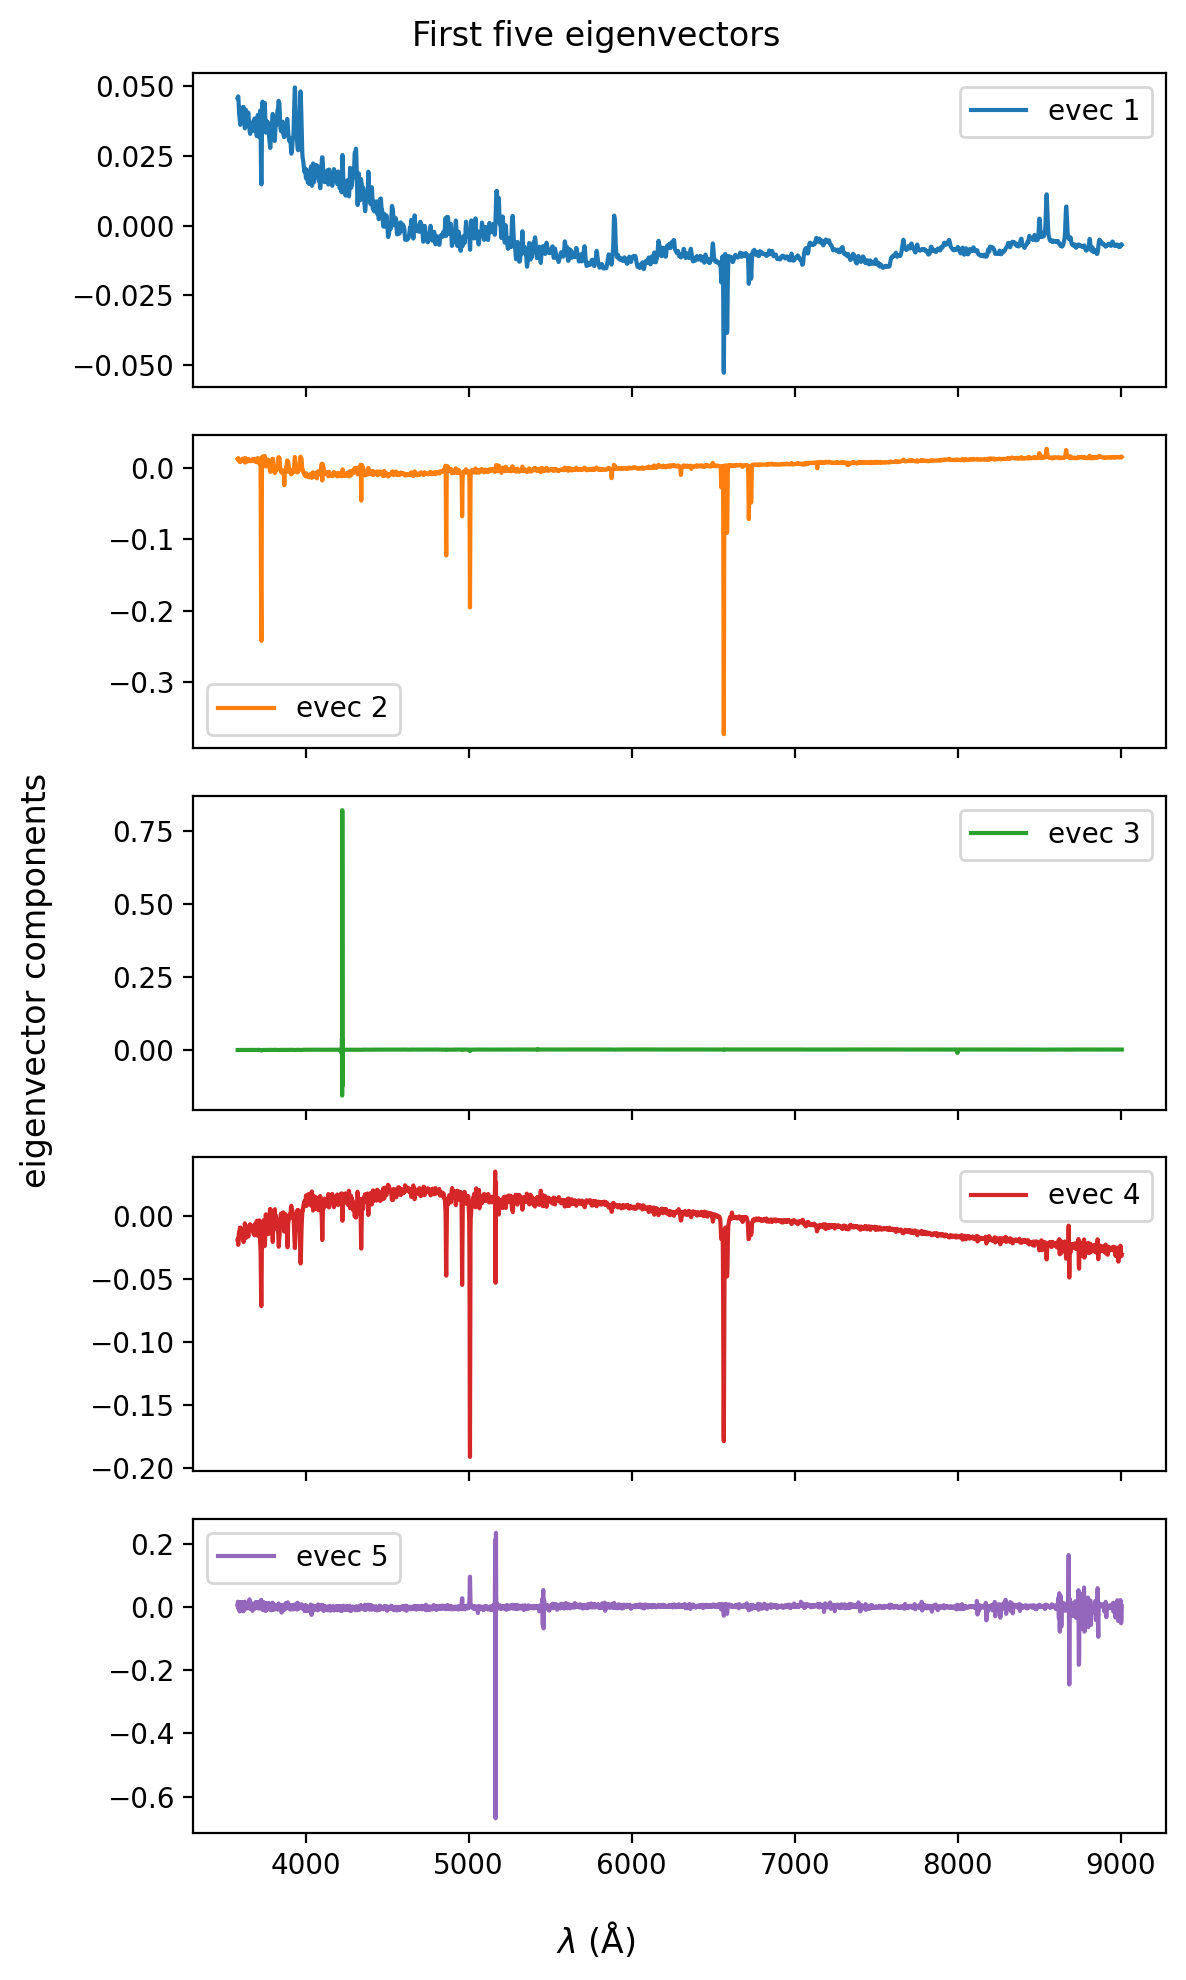
\includegraphics[scale = 0.65]{images/ps6-1d2.png}
    \caption{First five eigenvectors.}
    \label{fig:5evec}
\end{figure}

\subsection{Part (e)}
The first five eigenvectors of the covariance matrix computed using SVD are show in Figure \ref{fig:5evecSVD}.
\begin{figure}[H]
    \centering
    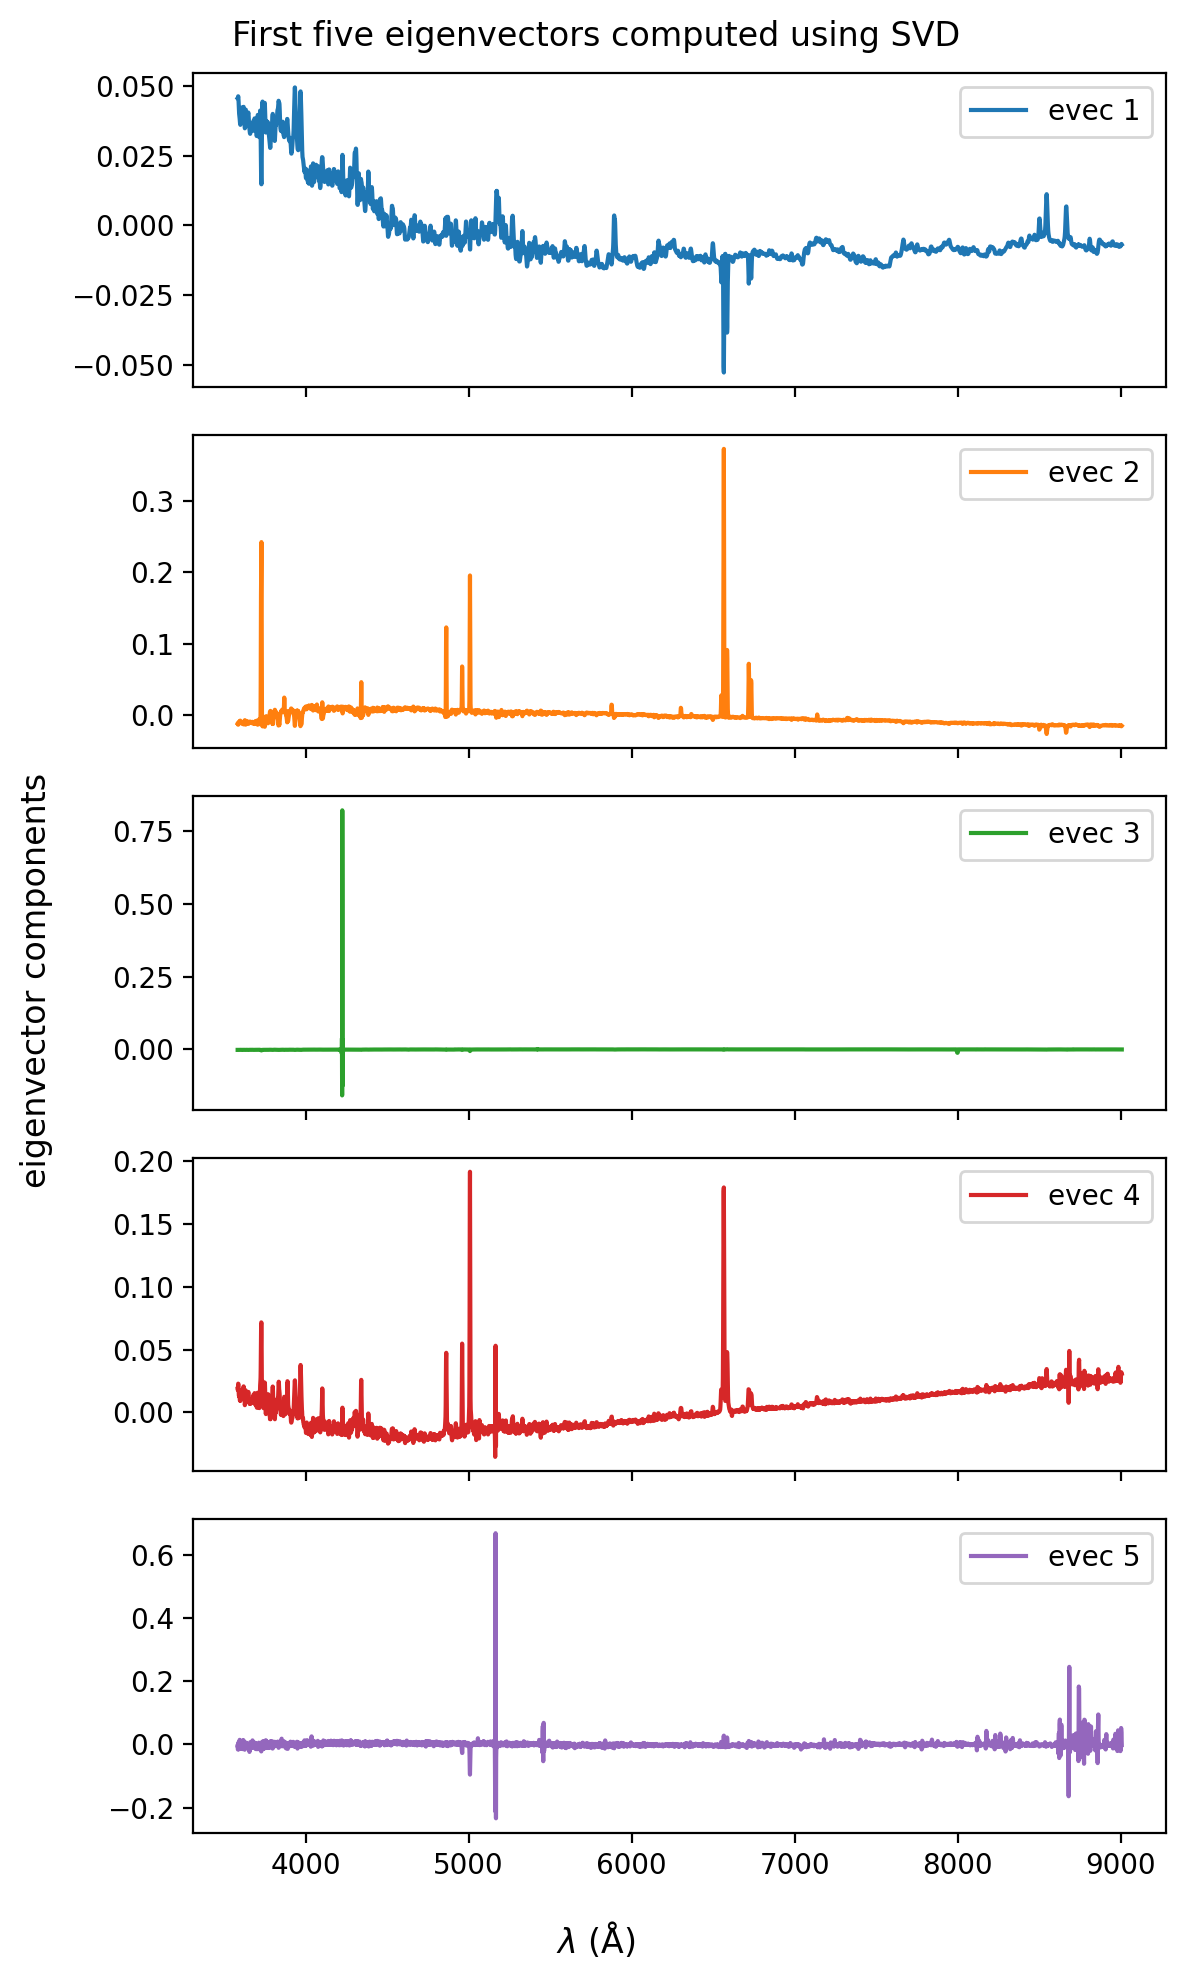
\includegraphics[scale = 0.65]{images/ps6-1e2.png}
    \caption{First five eigenvectors computed using SVD.}
    \label{fig:5evecSVD}
\end{figure}

\lstinputlisting[caption={Eigenvalues.}, label={lst:ev}]{code/ps6-1e.txt}

As shown in Listing \ref{lst:ev}, the eigenvalues computed using the two methods are the same, which indicates that the eigenvectors are equivalent. We note that eigenvectors 2, 4, and 5 in Figure \ref{fig:5evec} and Figure \ref{fig:5evecSVD} are negative to each other. But this is reasonable as one eigenvalue can associate with multiple eigenvectors that form an vector space known as eigenspace.

Listing \ref{lst:time} shows that using SVD is actually slower than directly finding the eigenvectors of the covariance matrix using \texttt{np.linalg.eig()}. Here, the units are seconds, and both methods are implemented twice in the shown time.
\lstinputlisting[caption={Computational cost.}, label={lst:time}]{code/ps6-1e2.txt}

\subsection{Part (f)}
Listing \ref{lst:condition} shows that the condition number of the covariance matrix \textbf{C} is quite large, whereas the condition number of the flux residue matrix \textbf{R} is much smaller. This might be one reason we want to use the SVD method.
\lstinputlisting[caption={Condition number.}, label={lst:condition}]{code/ps6-1f.txt}

\subsection{Part (g)}
Figure \ref{fig:approx} shows the approximated flux with $N_c = 5$ for galaxy number 2000.
\begin{figure}[H]
    \centering
    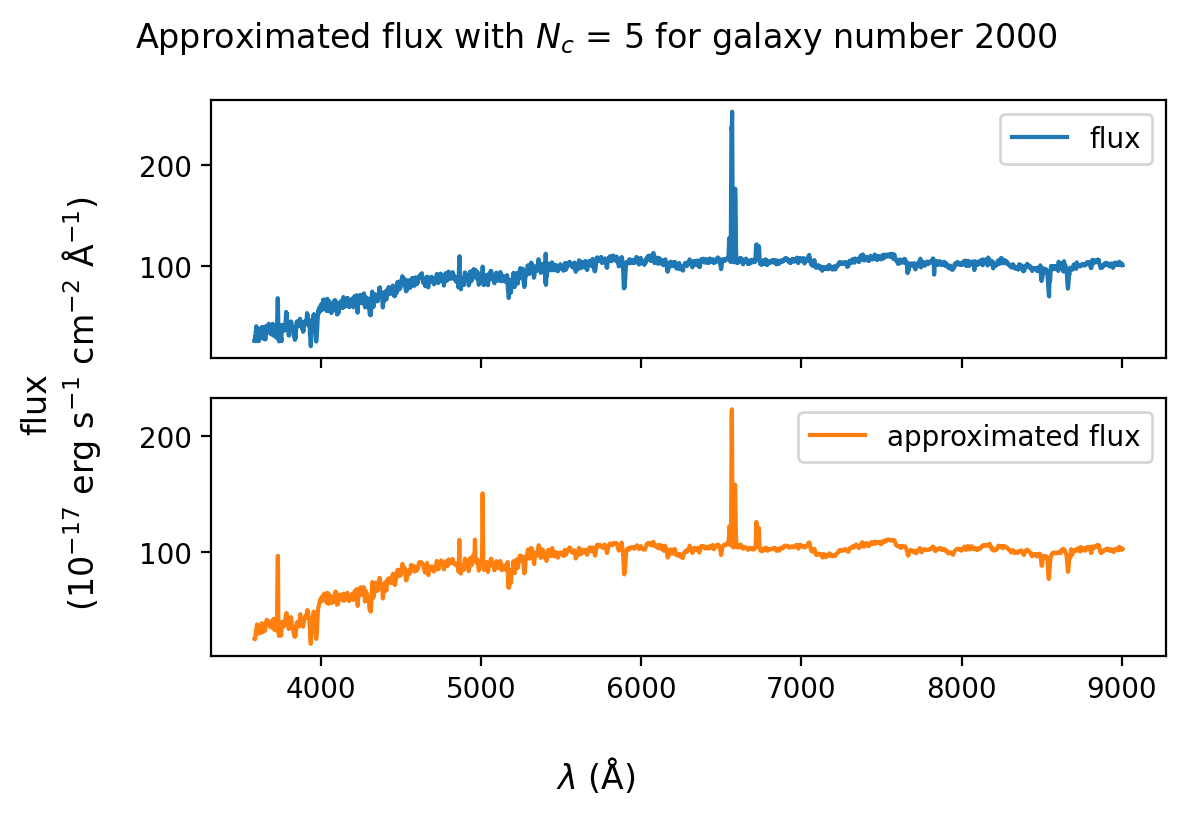
\includegraphics[scale = 0.75]{images/ps6-1g.png}
    \caption{Approximated flux with $N_c = 5$ for galaxy number 2000.}
    \label{fig:approx}
\end{figure}

\subsection{Part (h)}
Figure \ref{fig:3coeff} shows the first three coefficients $c_0$, $c_1$, and $c_2$.
\begin{figure}[H]
    \centering
    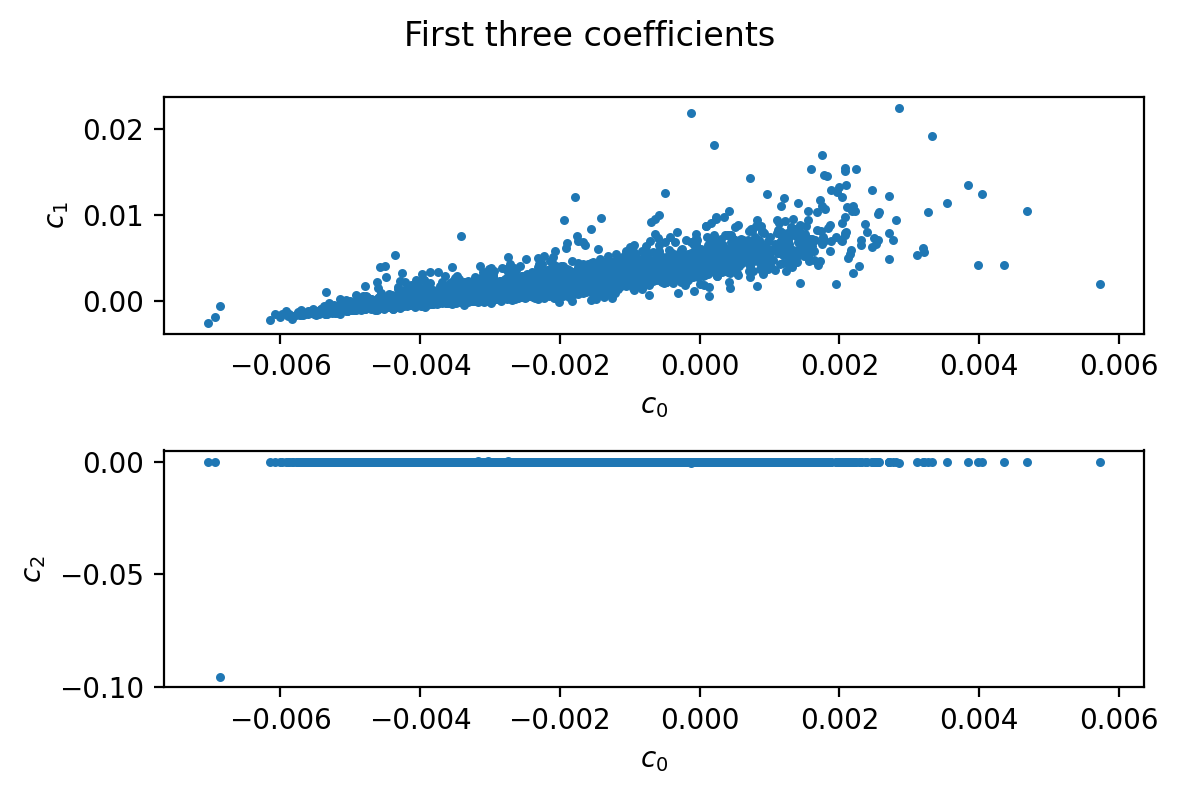
\includegraphics[scale = 0.75]{images/ps6-1h.png}
    \caption{First three coefficients.}
    \label{fig:3coeff}
\end{figure}

\subsection{Part (i)}
Figure \ref{fig:rms} shows the root mean square error of the approximated flux as a function of $N_c$.
\begin{figure}[H]
    \centering
    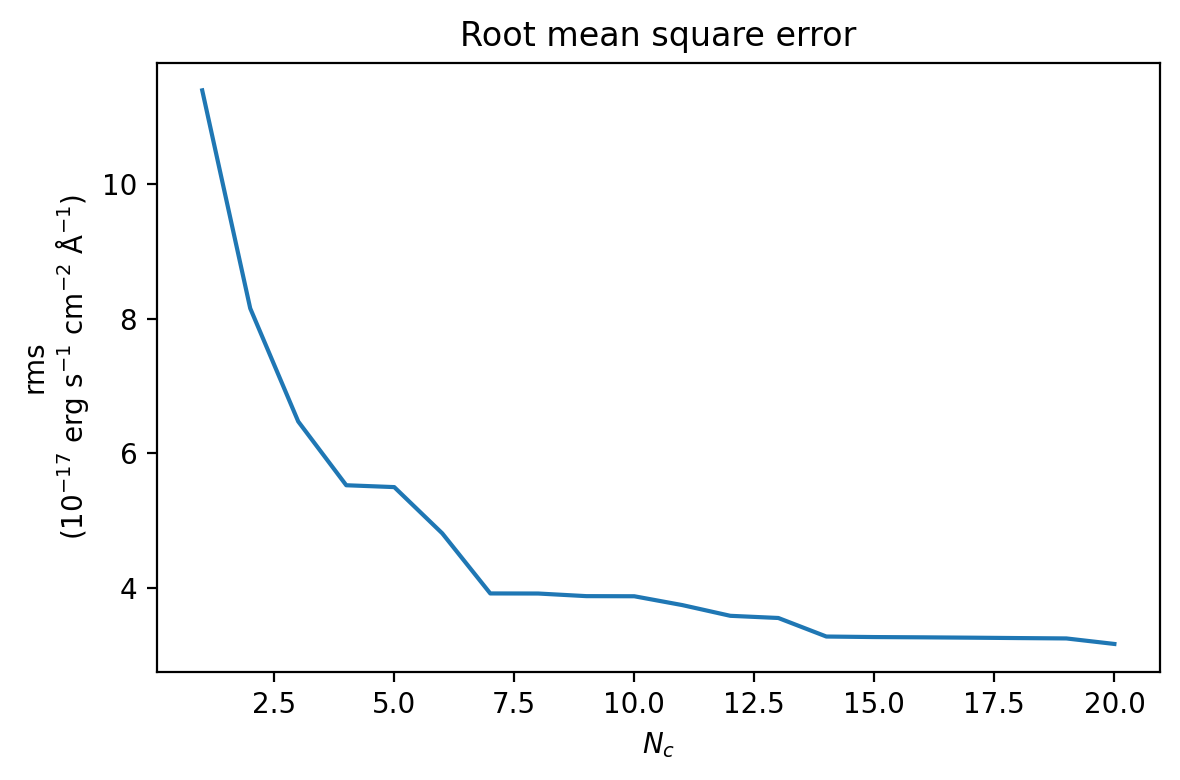
\includegraphics[scale = 0.75]{images/ps6-1i.png}
    \caption{Root mean square error.}
    \label{fig:rms}
\end{figure}

Listing \ref{lst:Nc20} shows the root mean square error for $N_c = 20$.
\lstinputlisting[caption={Root mean square error for $N_c = 20$.}, label={lst:Nc20}]{code/ps6-1i.txt}

\end{document}
